\section{  Logistic Regression}

\subsection{ Visualizing the data}

\begin{lstlisting}
import numpy as np
from matplotlib import pyplot as plt


def plotData(X,y):

	# ================= YOUR CODE HERE ===================
	# Instructions: Plot data X with different markers according the value in y
	# ====================================================

	pos = X[(y==1).flatten(),:]
	neg = X[(y==0).flatten(),:]
	plt.figure()
	plt.scatter(neg[:, 0], neg[:, 1], s=20, marker='P', color='b')
	plt.scatter(pos[:, 0], pos[:, 1], s=20, marker='o', color='r')
	plt.xlabel('Exam 1 score')
	plt.ylabel('Exam 2 score')
	plt.grid(True)
	plt.legend(['Not admitted (y=0)','Admitted (y=1)'], loc='upper right', shadow=True,fontsize='x-large', numpoints=1)
	plt.show()

	# =======================================

\end{lstlisting}

\begin{figure}[H]
    \centering
    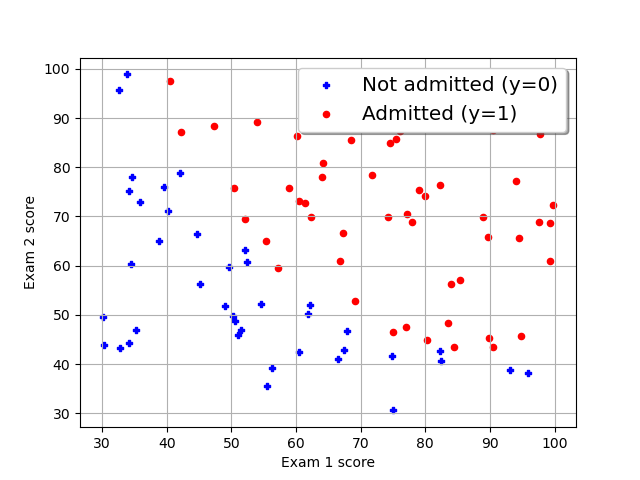
\includegraphics[width=0.75\linewidth]{figure/datas.png}
    \label{fig:placeholder}
\end{figure}

\subsection{Implementation}

\subsubsection{Sigmoid function}

\begin{lstlisting}
import numpy as np
from matplotlib import pyplot as plt


def plotData(X,y):

	# ================= YOUR CODE HERE ===================
	# Instructions: Plot data X with different markers according the value in y
	# ====================================================

	pos = X[(y==1).flatten(),:]
	neg = X[(y==0).flatten(),:]
	plt.figure()
	plt.scatter(neg[:, 0], neg[:, 1], s=20, marker='P', color='b')
	plt.scatter(pos[:, 0], pos[:, 1], s=20, marker='o', color='r')
	plt.xlabel('Exam 1 score')
	plt.ylabel('Exam 2 score')
	plt.grid(True)
	plt.legend(['Not admitted (y=0)','Admitted (y=1)'], loc='upper right', shadow=True,fontsize='x-large', numpoints=1)

	# =======================================

\end{lstlisting}

\subsubsection{Cost function and gradient}

\begin{lstlisting}
import numpy as np
from sigmoid import sigmoid

def costFunction(theta, X, y):
    """ computes the cost of using theta as the
    parameter for logistic regression."""

	# Initialize some useful values
    m,n = X.shape   # number of training examples and parameters
    theta = theta.reshape((n,1)) # due to the use of fmin_tnc

    
    # ============= YOUR CODE HERE ================
    # Instructions: Compute the cost of a particular choice of theta.
    #               You should set J to the cost.
    #
    arg1 = X @ theta
    arg2 = sigmoid(arg1)
    j = (-y*np.log(arg2) - (1-y)*np.log(1-arg2))   

    J = np.sum(j) / m

    # ==================================================
    
    return J

\end{lstlisting}



\begin{lstlisting}
from sigmoid import sigmoid
import numpy as np


def gradientFunction(theta, X, y):
    """
    Compute cost and gradient for logistic regression with regularization

    computes the cost of using theta as the parameter for regularized logistic 
    regression and the gradient of the cost w.r.t. to the parameters.
    """

    # Initialize some useful values
    # number of training examples 
    m = X.shape[0]   

    # number of parameters
    n = X.shape[1]   
    theta = theta.reshape((n,1)) # due to the use of fmin_tnc


    # gradient variable
    grad = 0.


    # ============== YOUR CODE HERE ================
    # Instructions: Compute the gradient of a particular choice of theta.
    #               Compute the partial derivatives and set grad to the partial
    #               derivatives of the cost w.r.t. each parameter in theta

    arg1 = X @ theta
    arg2 = sigmoid(arg1)
    grad = (X.T @ (arg2 - y)) / m


    # ========================================

    return grad

\end{lstlisting}

\subsubsection{Learning parameters using fmin tnc}

\begin{figure}[H]
    \centering

    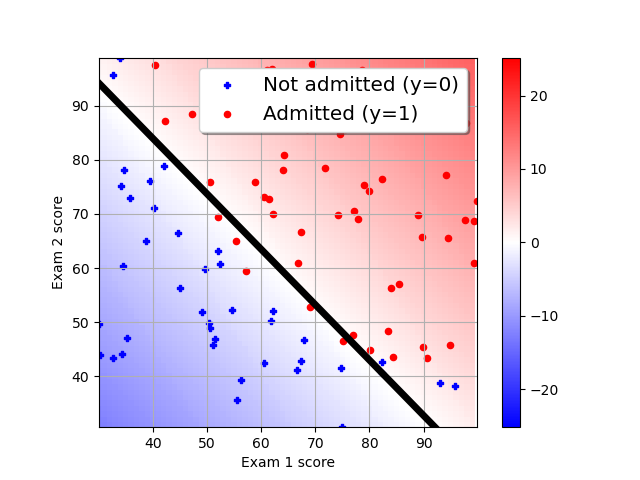
\includegraphics[width=0.75\linewidth]{figure/boundary.png}
    \label{fig:placeholder}
\end{figure}

The function plotDecisionBoundary.py takes the decision at the point where the sigmoid function is equal to 0.5, which is the same as saying that the logit function is equal to 0. Then we have theta0 + theta1*x1 + theta2*x2 = 0, which is a linear equation in x1 and x2. The function plotDecisionBoundary.py takes the two points where the line intersects the axes and plots the line between them.

\subsubsection{ Evaluating logistic regression }


\begin{lstlisting}
import numpy as np
from sigmoid import sigmoid


def predict(theta, X):

    """ computes the predictions for X using a threshold at 0.5
    (i.e., if sigmoid(theta'*x) >= 0.5, predict 1)
    """

    # initialisation
    p = 0

	# ==================== YOUR CODE HERE ==================
	# Instructions: Complete the following code to make predictions using
	#               your learned logistic regression parameters.
	#               You should set p to a vector of 0's and 1's
	#

    p = sigmoid(X @ theta) >= 0.5

	# ========================================================

    return np.atleast_2d(p).T

\end{lstlisting}




\begin{figure}[H]
    \centering

    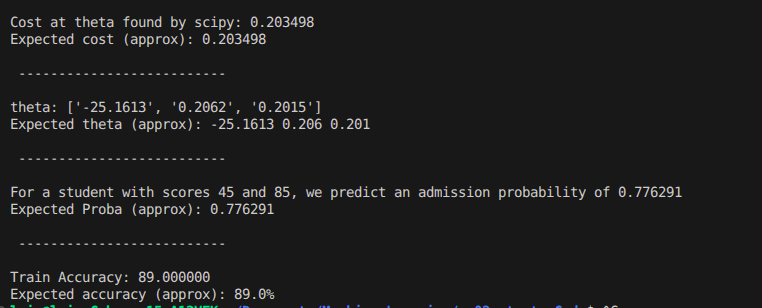
\includegraphics[width=0.75\linewidth]{figure/image.png}
    \label{fig:placeholder}
\end{figure}







\section{Regularized logistic regression}

\subsection{Visualizing the data}

\begin{figure}[H]
    \centering

    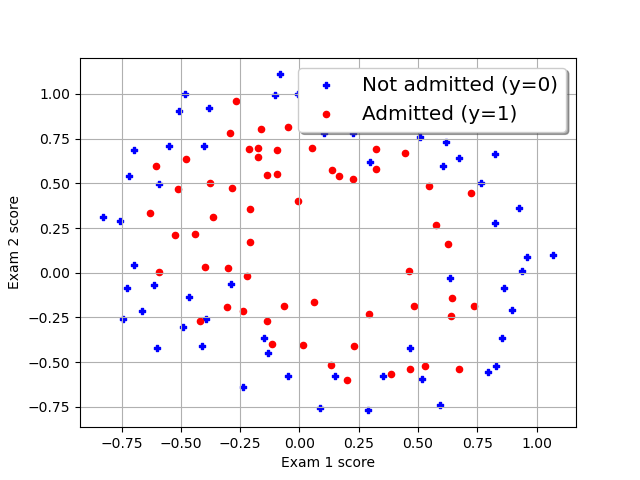
\includegraphics[width=0.75\linewidth]{figure/datas_reg.png}
    \label{fig:placeholder}
\end{figure}

\subsection{Feature mapping}

\subsection{Cost function and gradient} \label{subsec:cost}

\begin{lstlisting}
import numpy as np
from sigmoid import sigmoid


def costFunctionReg(theta, X, y, Lambda):
    """
    Compute cost and gradient for logistic regression with regularization

    computes the cost of using theta as the parameter for regularized logistic regression and the
    gradient of the cost w.r.t. to the parameters.
    """
    # Initialize some useful values
    m,n = X.shape   # number of training examples and parameters
    theta = theta.reshape((n,1)) # due to the use of fmin_tnc

    J = 0.

    # ================ YOUR CODE HERE ==============
    # Instructions: Compute the cost of a particular choice of theta.
    #               You should set J to the cost.
    #               Compute the partial derivatives and set grad to the partial
    #               derivatives of the cost w.r.t. each parameter in theta

    # =================================================
    
    arg1 = (X@theta)
    arg2 = sigmoid(arg1)
    J = (-1/m) * (y.T @ np.log(arg2) + (1-y).T @ np.log(1-arg2)) + (Lambda/(2*m))*np.sum(theta[1:]**2)  
    
    # ===========================================
    
    return J

\end{lstlisting}



\begin{lstlisting}
import numpy as np
from sigmoid import sigmoid


def gradientFunctionReg(theta, X, y, Lambda):
    """
    Compute cost and gradient for logistic regression with regularization

    computes the cost of using theta as the parameter for regularized logistic regression and the
    gradient of the cost w.r.t. to the parameters.
    """
    
    # Initialize some useful values
    m,n = X.shape   # number of training examples and parameters
    theta = theta.reshape((n,1)) # due to the use of fmin_tnc

    grad = 0.

    # ================ YOUR CODE HERE ================
    # Instructions: Compute the gradient of a particular choice of theta.
    #               Compute the partial derivatives and set grad to the partial
    #               derivatives of the cost w.r.t. each parameter in theta
    # ===============================================

    arg1 = (X@theta)
    arg2 = sigmoid(arg1)
    grad = (1/m) * (X.T @ (arg2 - y)) + (Lambda/m) * np.vstack([[0], theta[1:]])  


    # =============================================

    return grad
\end{lstlisting}


\subsubsection{Learning parameters using fmin tnc}

\begin{figure}[H]
	\centering
	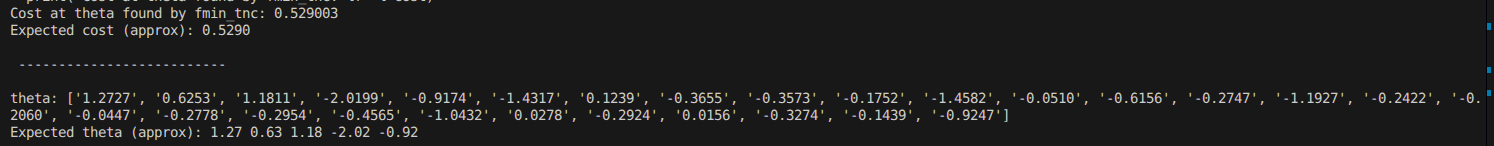
\includegraphics[width=0.75\linewidth]{figure/imagecopy.png}
	\label{fig:placeholder}
\end{figure}

\subsection{Plotting the decision boundary}

\begin{figure}[H]
	\centering

	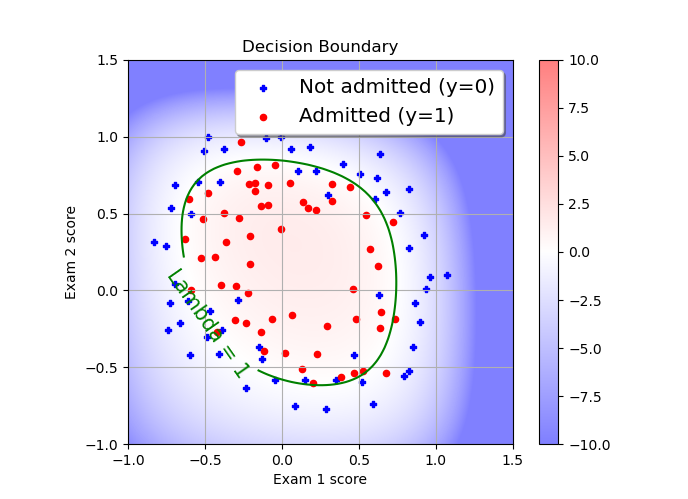
\includegraphics[width=0.75\linewidth]{figure/boundary-2.png}
	\label{fig:placeholder}
\end{figure}

\subsection{Impact of $\lambda$}

\begin{figure}[H]
    \centering
    % Première ligne
    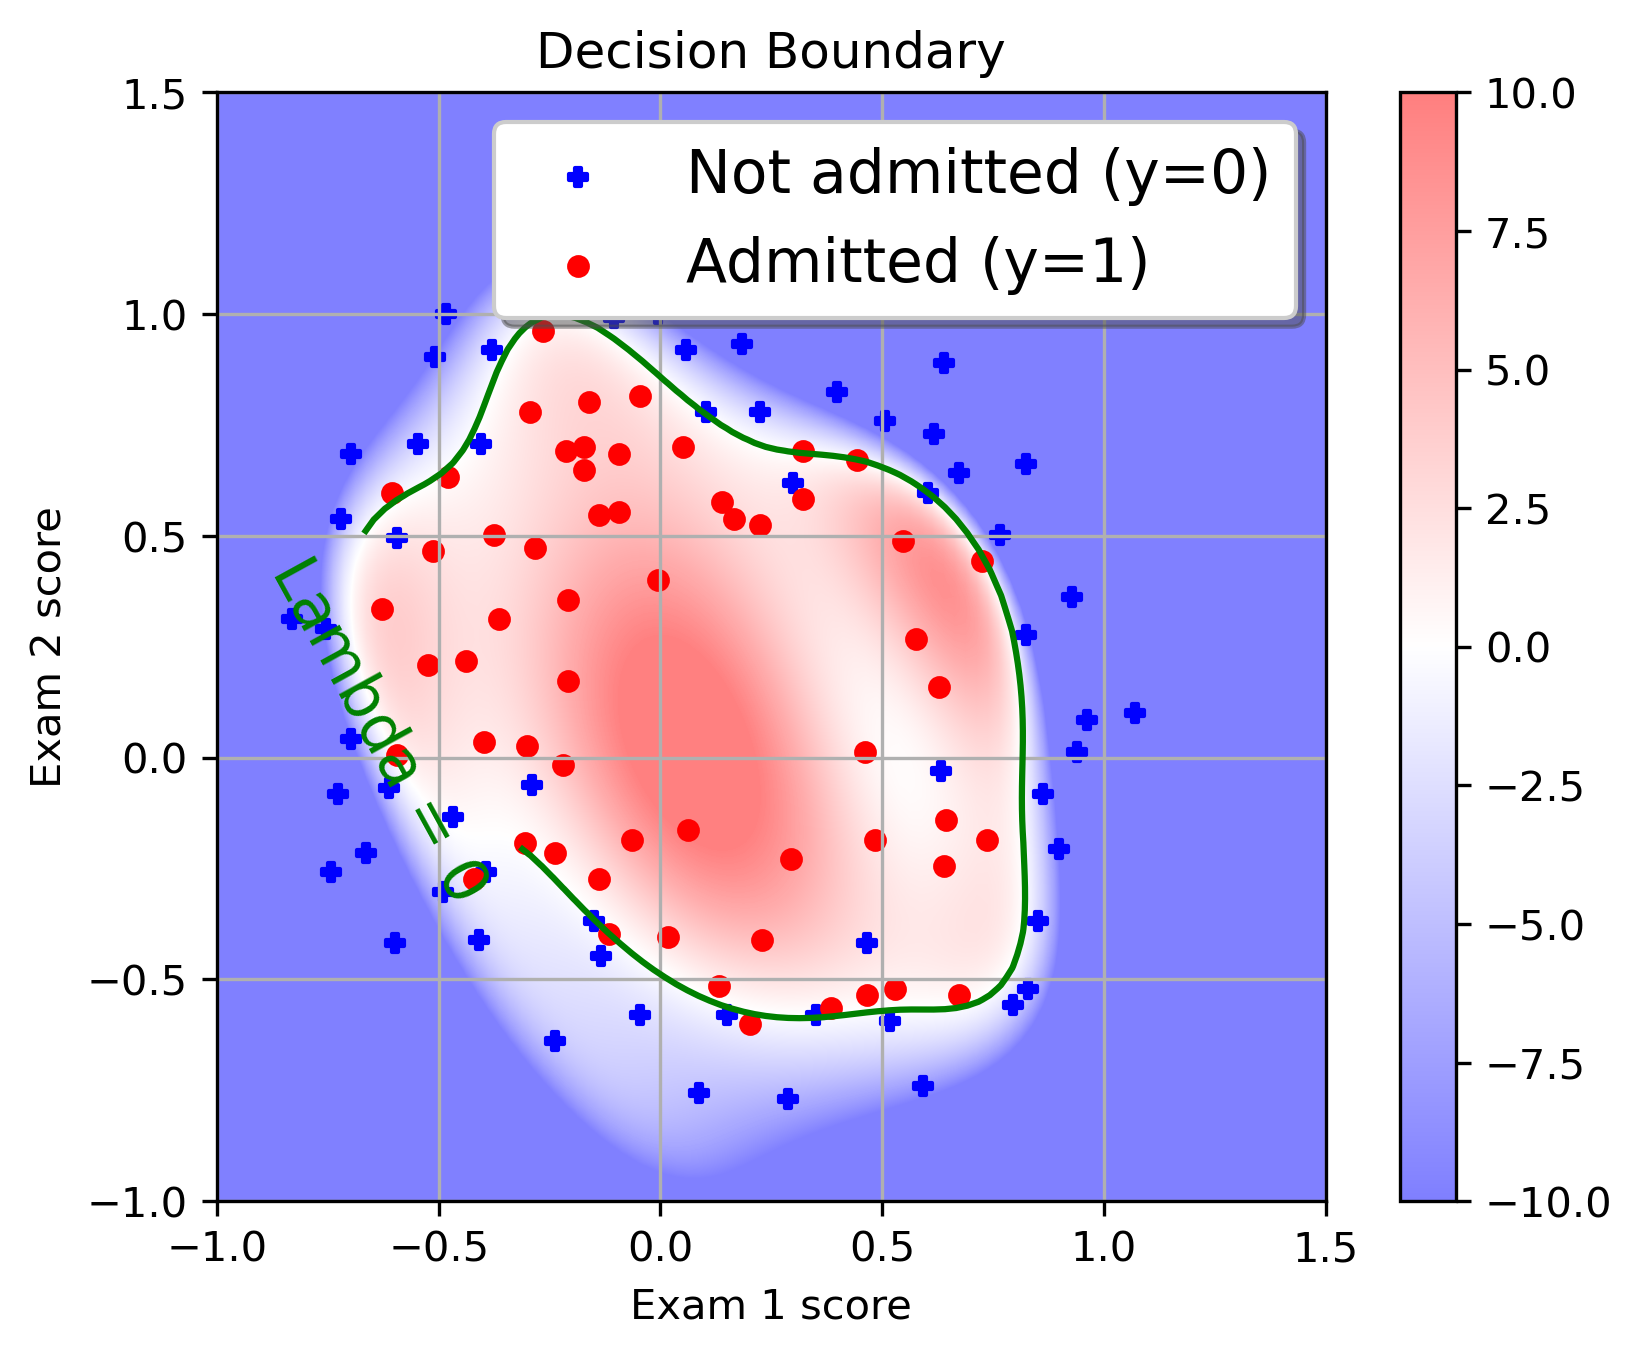
\includegraphics[width=0.45\linewidth]{figure/boundary_0.png}
    \hfill
    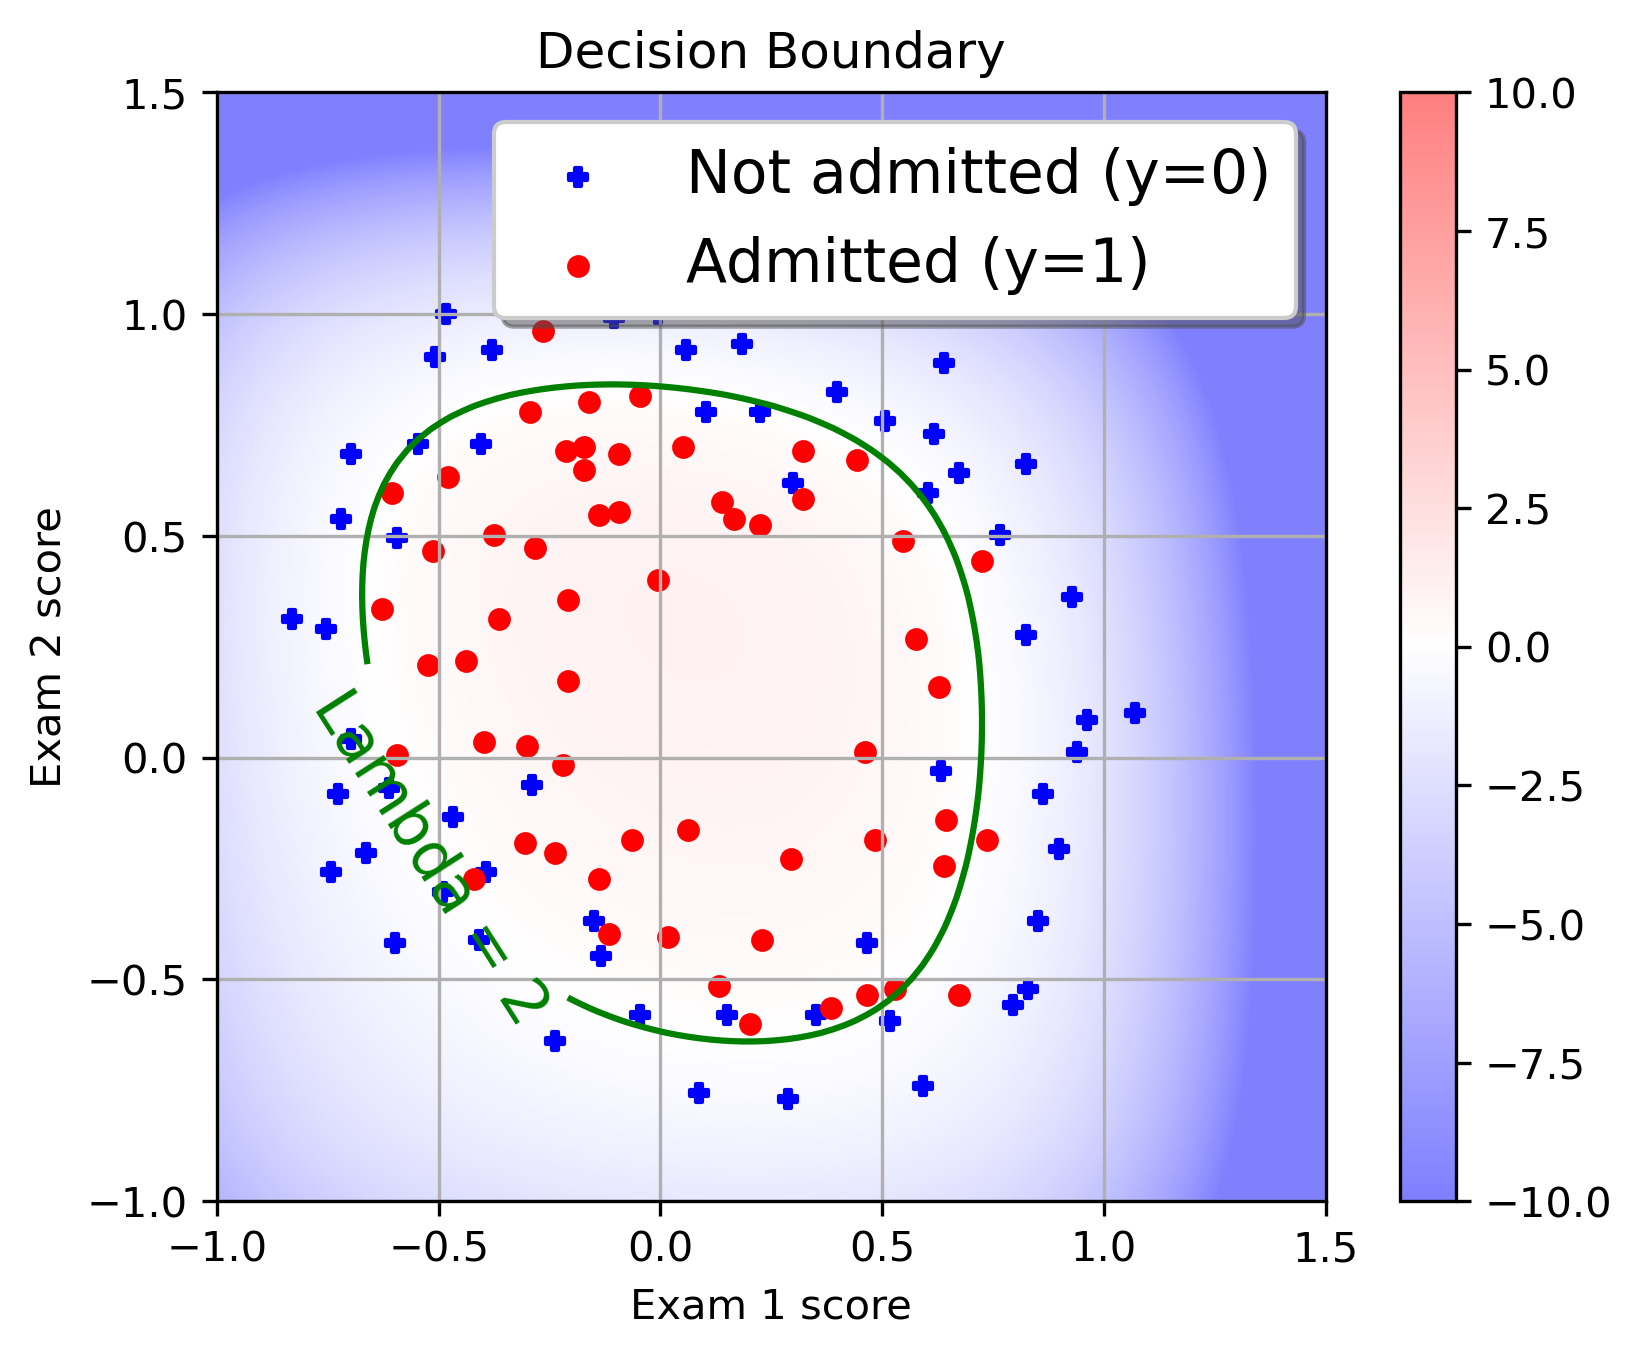
\includegraphics[width=0.45\linewidth]{figure/boundary_2.png}
    
    \vspace{0.5cm} % Un peu d'espace entre les deux lignes
    
    % Deuxième ligne
    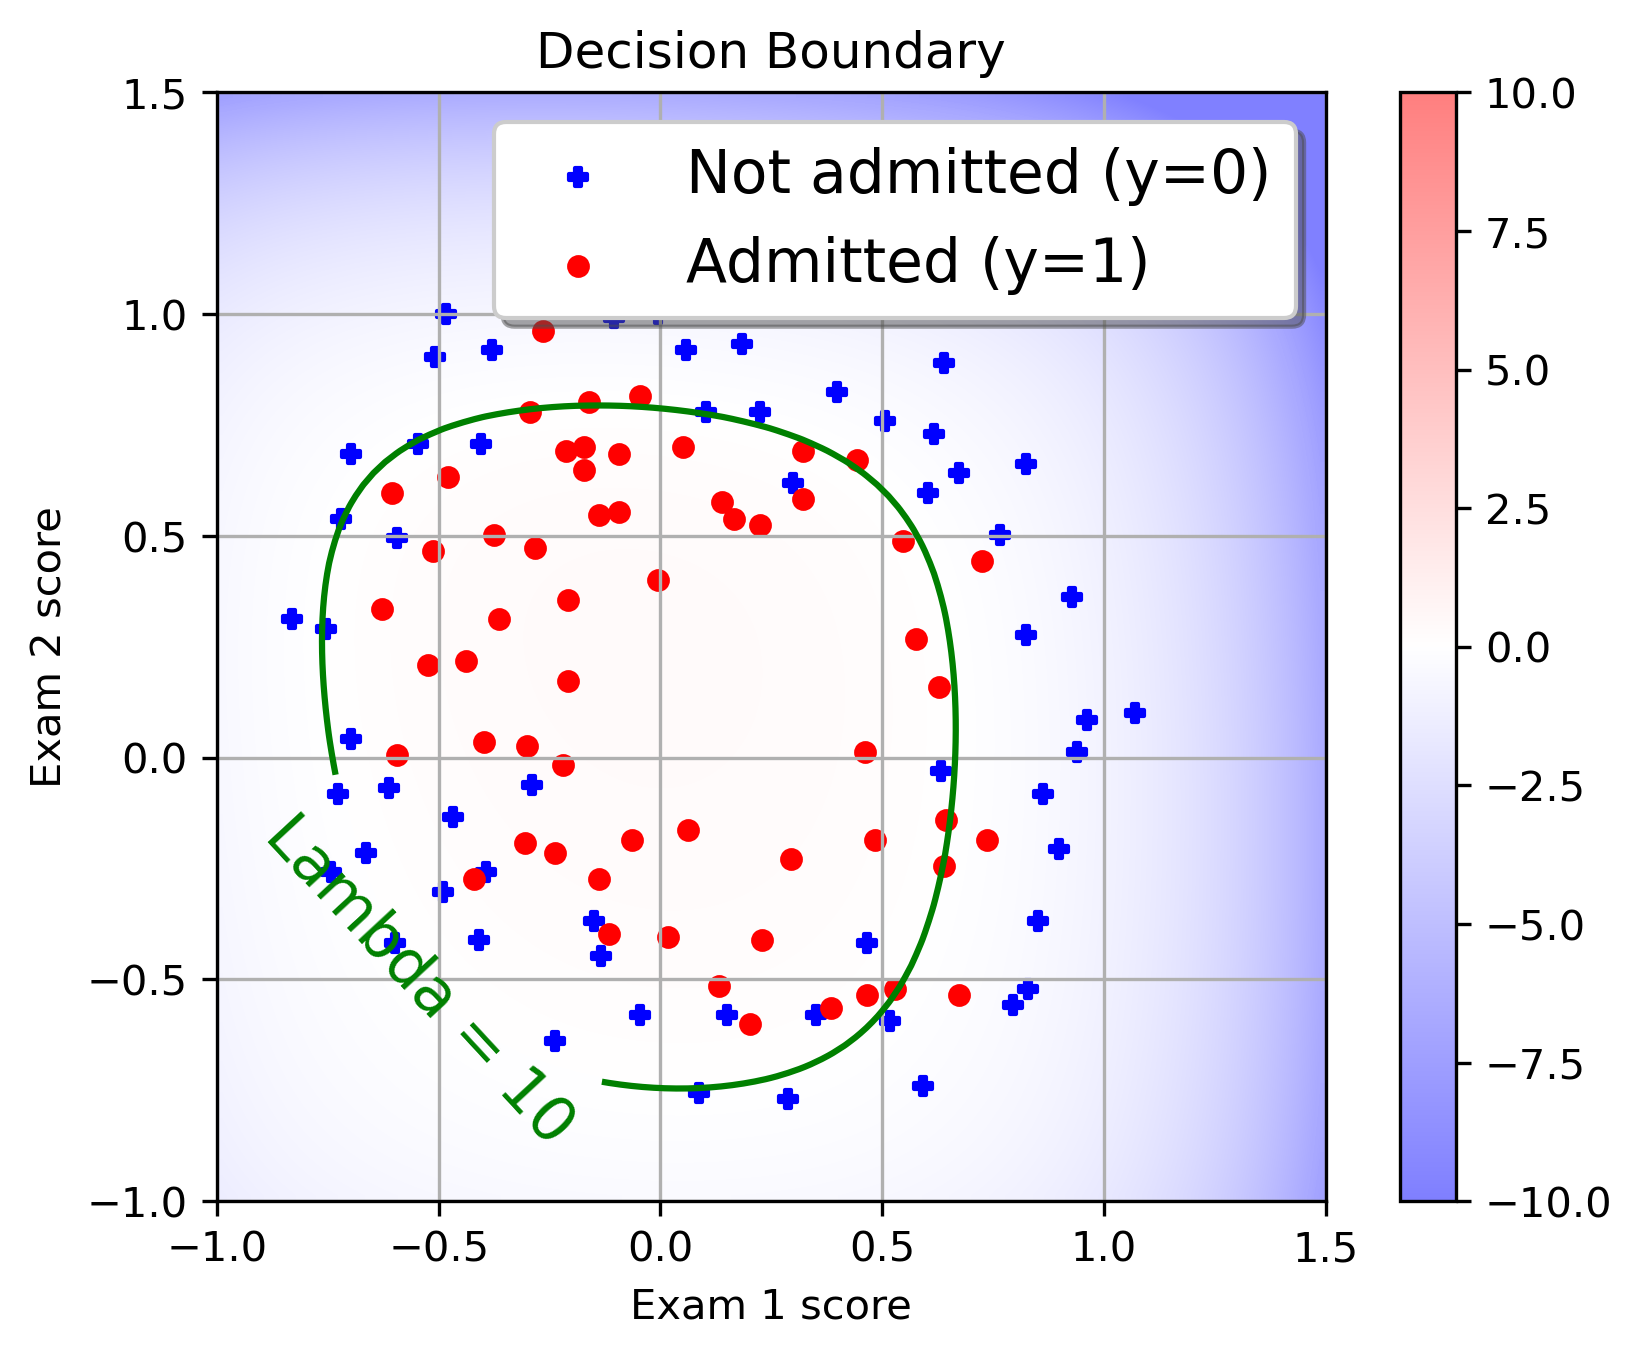
\includegraphics[width=0.45\linewidth]{figure/boundary_10.png}
    \hfill
    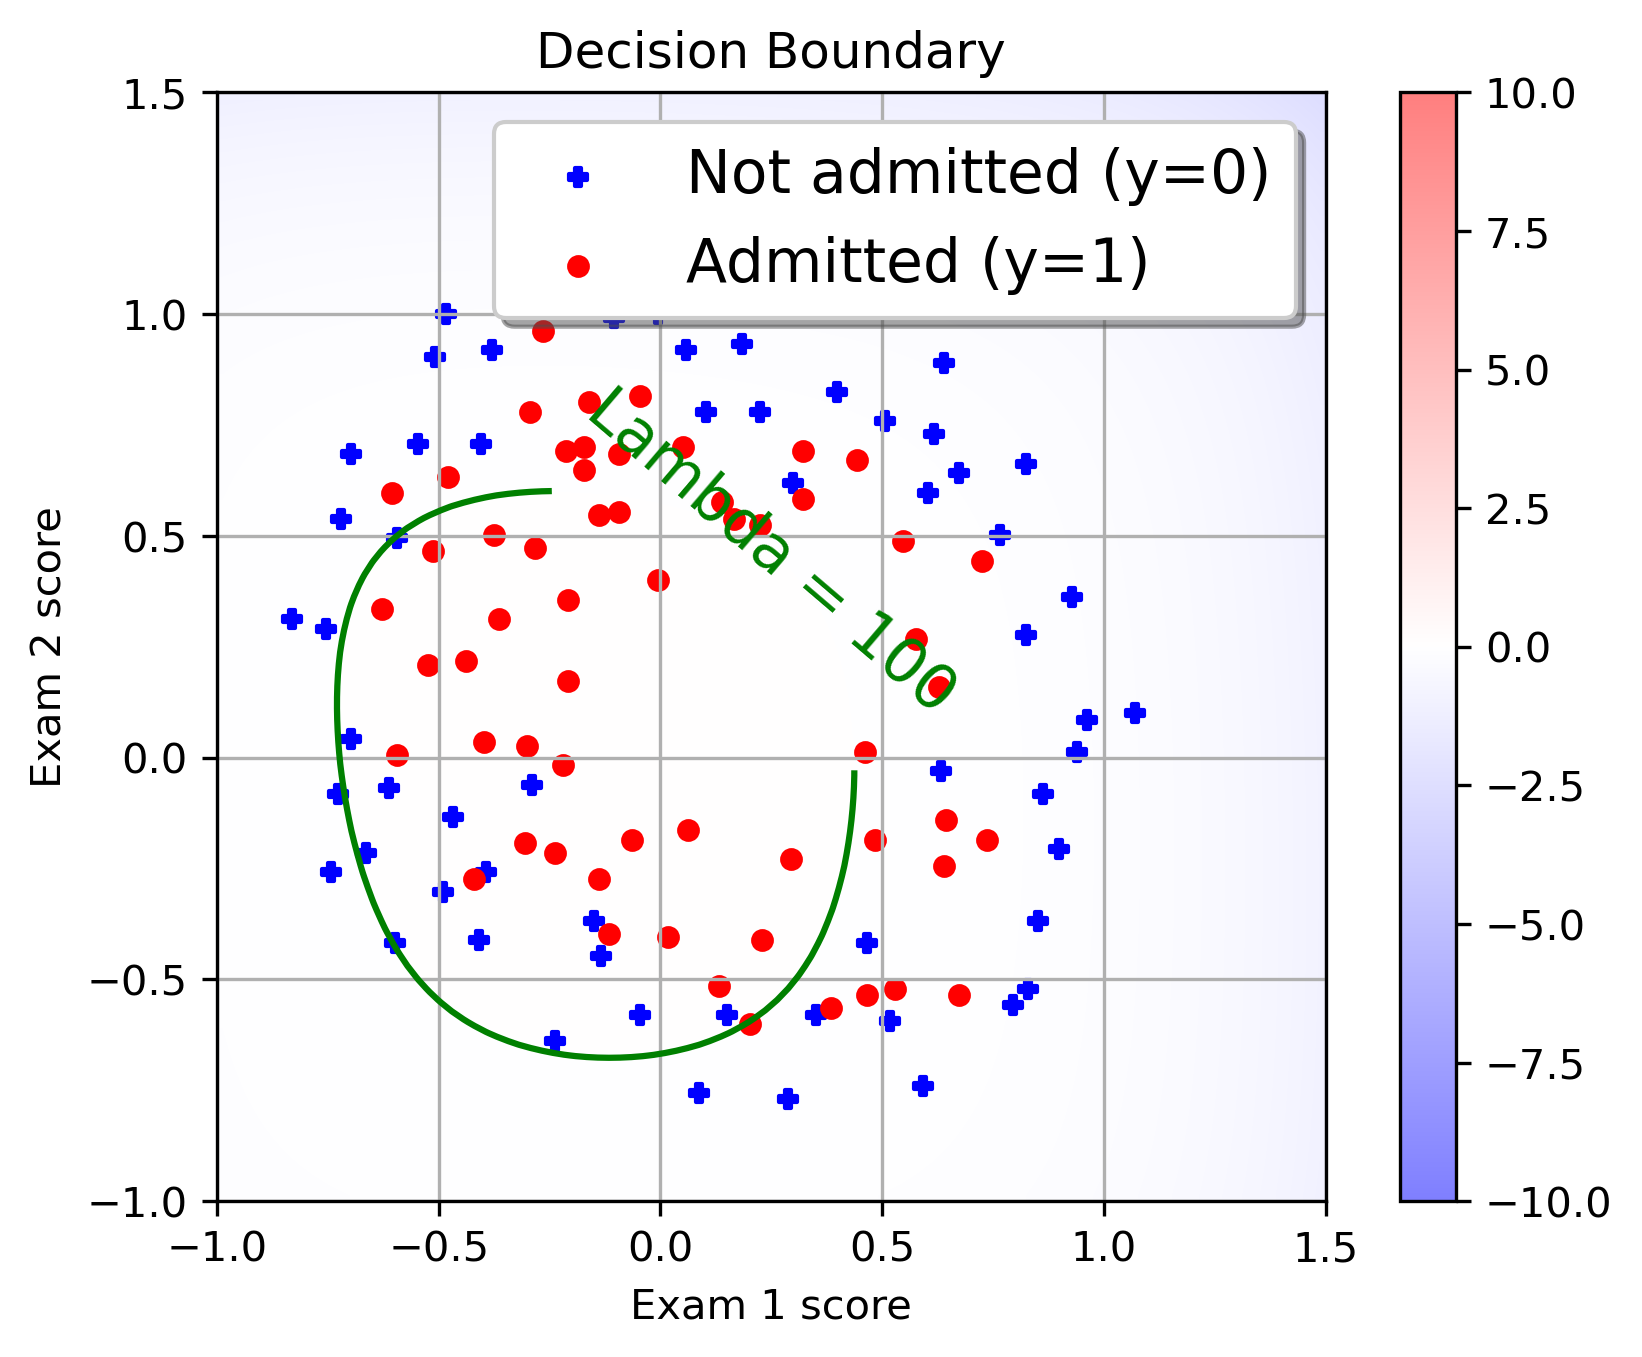
\includegraphics[width=0.45\linewidth]{figure/boundary_100.png}
    
    \caption{Évolution de la frontière de décision selon la valeur de Lambda.}
    \label{fig:boundaries}
\end{figure}





\section{Multi-class classification}

\subsection{Dataset}

\subsection{Visualizing the data}

\begin{figure}[H]
    \centering
    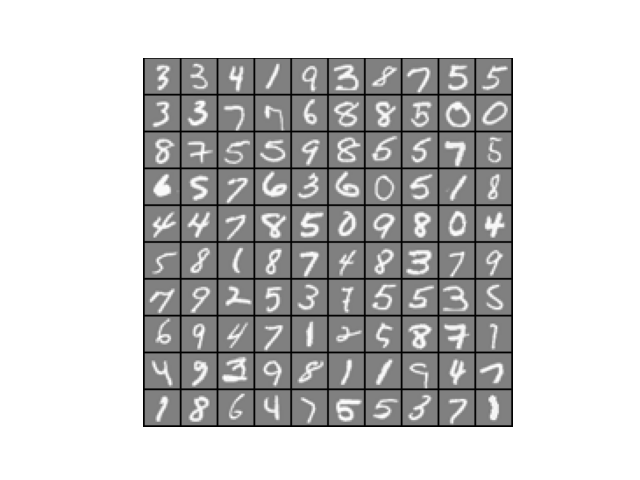
\includegraphics[width=0.75\linewidth]{figure/multiclass.png}
    \label{fig:placeholder}
\end{figure}

\subsection{Vectorizing Logistic Regression}
\subsubsection{Vectorizing the cost function}
The code is descdribed in the subsection \ref{subsec:cost}.
\subsubsection{Vectorizing the gradient}
The code is descdribed in the subsection \ref{subsec:cost} as well.

\subsection{ Learning a one-vs-all classifier}

\subsection{One-vs-all prediction}


\begin{lstlisting}
import numpy as np

from sigmoid import sigmoid

def predictOneVsAll(all_theta, X):
    
    """will return a vector of predictions
    for each example in the matrix X. Note that X contains the examples in
    rows. all_theta is a matrix where the i-th row is a trained logistic
    regression theta vector for the i-th class. You should set p to a vector
    of values from 1..K (e.g., p = [1 3 1 2] predicts classes 1, 3, 1, 2
    for 4 examples) """

# ================= YOUR CODE HERE =================
# Instructions: Complete the following code to make predictions using
#               your learned logistic regression parameters (one-vs-all).
#               You should set p to a vector of predictions (from 1 to
#               num_labels).
#
# Hint: This code can be done all vectorized using the max function.
#       In particular, the np.argmax function can return the index of the max 
#       element, for more information see 'numpy.argmax' on the numpy website. 
#       If your examples are in rows, then, you can use 
#       np.argmax(probs, axis=1) to obtain the max for each row.
#       

    p = np.argmax(sigmoid(X @ all_theta.T), axis=1) 



# ===============================================

    return np.atleast_2d(p).T 
\end{lstlisting}

\subsection{Some questions, you have to answer...}

\begin{enumerate}
    \item Identifiez les différences d’approches entre le TP1 et le TP2 et les différences de résolution du
problème.

    \subitem Dans la TP1, on a fait de la régression linéaire. Le but était de deviner une valeur exacte et continue comme le prix d'une maison. Dans le TP2, on a fait de la classification. Le but n'étais plus de trouver un chiffre mais de classer des données dans des catégories, comme dire "oui" ou "non" (admis ou refusé).
Dans le TP1, on a écrit nous mêmes tout le code pour faire avancer l'ordinateur pas à pas et trouver l'erreur minimum. Dans le TP2 on a utilisé une fonction Python déjà prête la fmin\_tnc qui fait tout ce travail d'optimisation toute seule. On a juste eu à lui donner la fonction pour calculer l'erreur (le coût) et le gradient.

    \item A quoi sert le principe de régularisation ?
    \subitem La régularisation sert à empêcher le modèle d'être trop complexe. Quand on donne beaucoup d'informations à l'ordinateur il a tendance à vouloir apprendre les données d'entraînement par cœur, avec tous leurs petits défauts. La régularisation le force à garder des calculs plus simples pour qu'il reste capable de bien juger de nouvelles données qu'il n'a jamais vues.

     \item Décrivez le problème du sur-apprentissage et comment on y répond dans ce TP. Quelle est l’influence
de la valeur de $\lambda$?
    \subitem Le sur-apprentissage (ou overfitting), c'est quand l'algorithme devient trop perfectionniste. Il dessine une frontière complètement tordue pour passer exactement sur chaque point d'entraînement.
                La solution dans le TP on utilise la régularisation pour pénaliser l'ordinateur s'il fait des courbes trop compliquées. C'était possible de remarqué que si $\lambda$ est trop petit, on laisse faire l'ordinateur et on a du sur-apprentissage . Si $\lambda$ est trop grand (comme 100), on punit trop le modèle et il ne fait plus d'efforts (c'est le sous-apprentissage). Le but est de trouver un $\lambda$ moyen pour avoir une courbe douce et naturelle.

    \item Dans quelles circonstances et pour quelles raisons utilise-t-on l’approche multiclasse ? Quelles sont
les différentes possibilités pour cette approche?
    \subitem On l'utilise quand on a plus de deux choix possibles à la fin. La régression logistique normale ne sait répondre que par "oui" ou "non" (2 choix). Mais pour lire des numéros de codes postaux on doit deviner un chiffre entre 0 et 9 (10 choix). On est obligé d'adapter la méthode.
            
    Une approche est un contre tous (One-vs-All). C'est ce qu'on a fait dans le TP. On entraîne le programme à séparer une seule catégorie de toutes les autres réunies par exemple : "est-ce un 3, ou est-ce que ce n'est pas un 3 ?", et on répète ça pour chaque chiffre.
\end{enumerate}